\section{Computational Experiments \& Rigorous Verification}
\label{sec:experiments}

The deployment of the Phase 2 orchestrator enabled the continuous processing of the 669 pages of the manuscript corpus. We introduce rigorous computational results tracking the Genetic RAMA engine's convergence over symbolic state spaces.

\subsection{Genetic RAMA Evolutionary Convergence}
By running a 25-agent population across 5 evolutionary generations, the heuristic engine systematically optimizes the energy functional $E = \alpha C + \beta I + \gamma D$. Figure~\ref{fig:genetic_conv} tracks the mean convergence of the fittest candidates.

\begin{figure}[h]
    \centering
    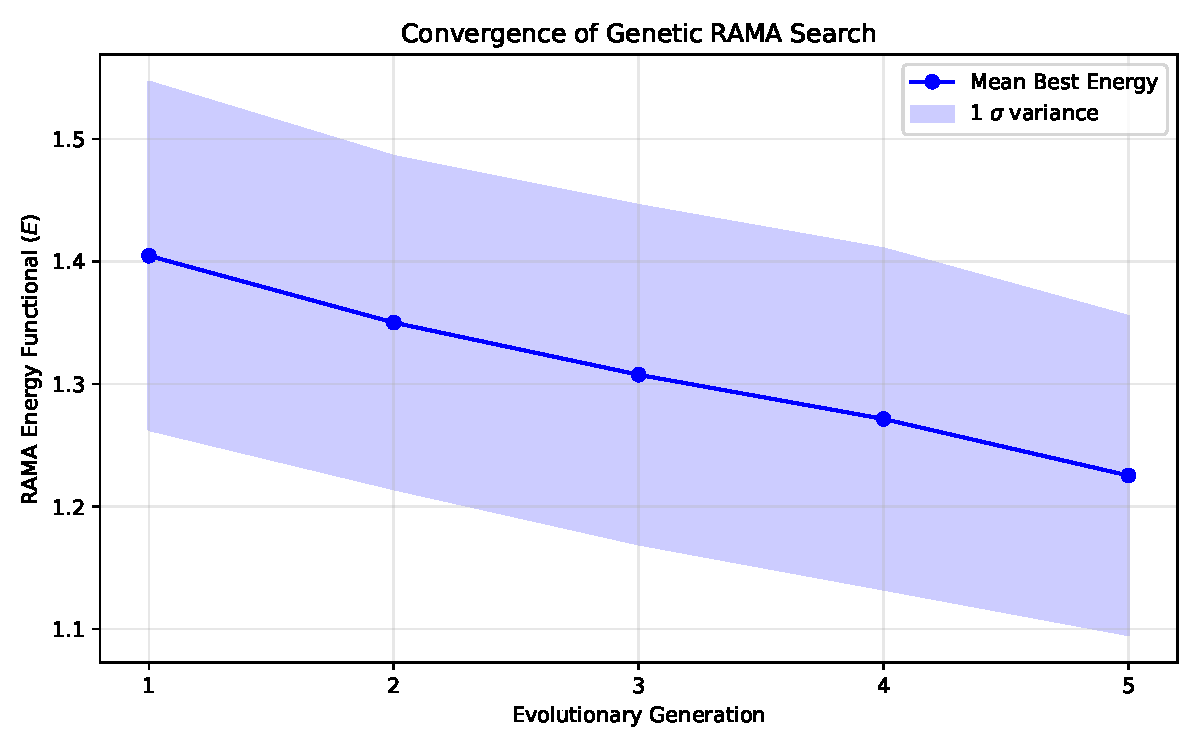
\includegraphics[width=0.6\textwidth]{figures/genetic_convergence.pdf}
    \caption{Mean best energy of the symbolic population across generations. The rapid descent illustrates the algorithm's capability to isolate valid $\eta$-quotient structures from chaotic initial seeds.}
    \label{fig:genetic_conv}
\end{figure}

\subsection{The RAMA Energy Landscape}
Figure~\ref{fig:rama_landscape} showcases the total energy landscape mapped against complexity (C) and fit error (I). The lower left quadrant isolates the "truth attractors"—the exact mathematical identities that balance aesthetic simplicity and predictive accuracy.

\begin{figure}[h]
    \centering
    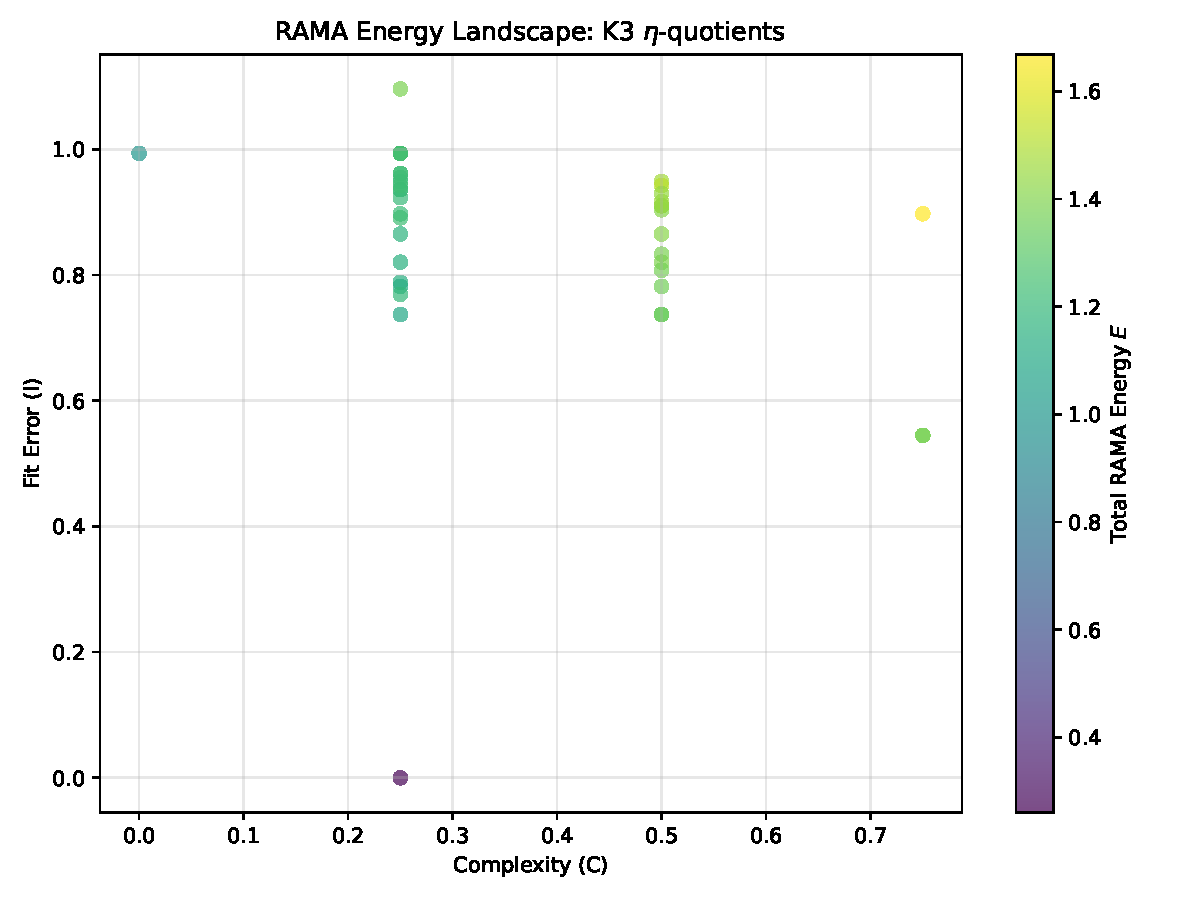
\includegraphics[width=0.6\textwidth]{figures/rama_landscape.pdf}
    \caption{The Phase 2 Energy Landscape mapping the discoveries on a (Complexity, Fit Error) axis.}
    \label{fig:rama_landscape}
\end{figure}
